
\documentclass{article}
\usepackage{lmodern}
\usepackage[T1]{fontenc}
\usepackage{shapepar}
\usepackage{microtype}
\usepackage{lipsum}
\usepackage{pgfplots}
\pgfplotsset{compat=1.9}
\usepackage{tikz}
\usetikzlibrary{calc,fit,intersections,folding}
\usepackage{pstricks-add}
\usetikzlibrary{arrows.meta,angles,arrows,quotes,backgrounds,calc}
\usepackage[left = 5mm, right = 5mm, top = 5mm, bottom = 5mm, a3paper, landscape]{geometry}

\usepackage{xstring}

\newcommand{\bound}{
\begin{tikzpicture}[scale = 0.29, xscale = 1.3]
    \fill[white] (0,1) -- (1,1) -- (1,3) -- (0,3) -- cycle;
\end{tikzpicture}
}

\newcommand{\tube}[1]{
\begin{tikzpicture}[scale = 0.22]
    \IfSubStr{#1}{a}{ \fill[blue, draw] (0,3) circle (8pt); }{ \draw (0,3) circle (8pt); }
    \IfSubStr{#1}{b}{ \fill[blue, draw] (0,2) circle (8pt); }{ \draw (0,2) circle (8pt); }
    \IfSubStr{#1}{c}{ \fill[blue, draw] (0,1) circle (8pt); }{ \draw (0,1) circle (8pt); }
    \IfSubStr{#1}{x}{ \fill[blue, draw] (1,3) circle (8pt); }{ \draw (1,3) circle (8pt); }
    \IfSubStr{#1}{y}{ \fill[blue, draw] (1,2) circle (8pt); }{ \draw (1,2) circle (8pt); }
    \IfSubStr{#1}{z}{ \fill[blue, draw] (1,1) circle (8pt); }{ \draw (1,1) circle (8pt); }
\end{tikzpicture}
}

\setlength{\parindent}{0em}

\newcommand{\clrone}{blue}
\newcommand{\clrtwo}{red}

\begin{document}
\thispagestyle{empty}

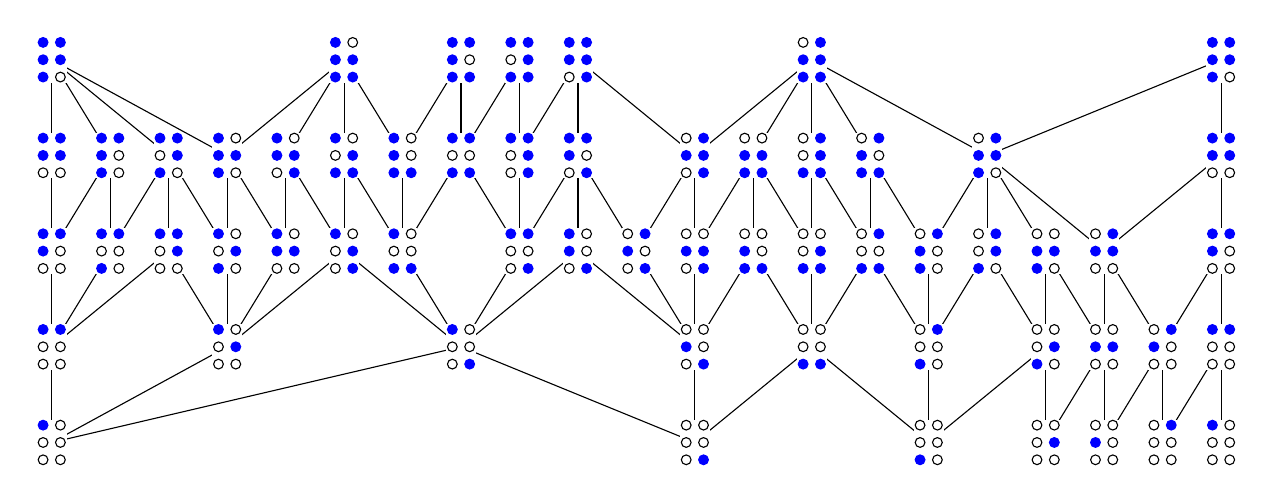
\begin{tikzpicture}[scale = 1.35,yscale = 0.9,xscale = 0.55]

\coordinate (a) at (3,0);
\coordinate (b) at (21,0);
\coordinate (c) at (18,0);
\coordinate (x) at (22,0);
\coordinate (y) at (20,0);
\coordinate (z) at (14,0);
\coordinate (ae) at (23,0);

\coordinate (ax) at (3,1);
\coordinate (ay) at (6,1);
\coordinate (az) at (10,1);
\coordinate (bz) at (14,1);
\coordinate (cz) at (16,1);
\coordinate (cx) at (18,1);
\coordinate (cy) at (20,1);
\coordinate (by) at (21,1);
\coordinate (bx) at (22,1);
\coordinate (axe) at (23,1);

\coordinate (abx) at (3,2);
\coordinate (acx) at (4,2);
\coordinate (axy) at (5,2);
\coordinate (acy) at (6,2);
\coordinate (aby) at (7,2);
\coordinate (ayz) at (8,2);
\coordinate (acz) at (9,2);
\coordinate (axz) at (11,2);
\coordinate (abz) at (12,2);
\coordinate (bxz) at (13,2);
\coordinate (byz) at (14,2);
\coordinate (bcz) at (15,2);
\coordinate (cyz) at (16,2);
\coordinate (cxz) at (17,2);
\coordinate (bcx) at (18,2);
\coordinate (cxy) at (19,2);
\coordinate (bcy) at (20,2);
\coordinate (bxy) at (21,2);
\coordinate (abxe) at (23,2);

\coordinate (abxy) at (3,3);
\coordinate (abcx) at (4,3);
\coordinate (acxy) at (5,3);
\coordinate (abcy) at (6,3);
\coordinate (abyz) at (7,3);
\coordinate (acyz) at (8,3);
\coordinate (abcz) at (9,3);
\coordinate (acxz) at (10,3);
\coordinate (axyz) at (11,3);
\coordinate (abxz) at (12,3);
\coordinate (bxyz) at (14,3);
\coordinate (bcyz) at (15,3);
\coordinate (cxyz) at (16,3);
\coordinate (bcxz) at (17,3);
\coordinate (bcxy) at (19,3);
\coordinate (abxye) at (23,3);

\coordinate (abcxy) at (3,4);
\coordinate (abcyz) at (8,4);
\coordinate (abcxz) at (10,4);
\coordinate (acxyz) at (11,4);
\coordinate (abxyz) at (12,4);
\coordinate (bcxyz) at (16,4);
\coordinate (abcxye) at (23,4);

\foreach \a/\b in {abx/abxy,a/ax,a/ay,a/az,z/az,z/bz,z/cz,c/cz,c/cx,c/cy,y/cy,y/by,b/by,b/bx,x/bx,x/axe,ae/axe,ax/abx,ax/acx,ax/axy,ay/axy,ay/acy,ay/aby, ay/ayz,az/ayz,az/acz,az/axz,az/abz,bz/abz,bz/bxz,bz/byz,bz/bcz,cz/bcz,cz/cyz,cz/cxz,cx/cxz,cx/bcx,cx/cxy,cy/cxy,cy/bcy,by/bcy,by/bxy,bx/bxy,bx/abxe,axe/abxe,abx/abcx,acx/abcx,acx/acxy,axy/acxy,acy/acxy,acy/abcy,aby/abcy,aby/abyz,ayz/abyz,ayz/acyz,acz/acyz,acz/abcz,acz/acxz,axz/acxz,axz/axyz,axz/abxz,abz/abxz,bxz/abxz,bxz/bxyz,byz/bxyz,byz/bcyz,bcz/bcyz,cyz/bcyz,cyz/cxyz,cxz/cxyz,cxz/bcxz,bcx/bcxz,bcx/bcxy,cxy/bcxy,bcy/bcxy,bxy/bcxy,bxy/abxye,abxy/abcxy,abcx/abcxy,acxy/abcxy,abcy/abcxy,abcy/abcyz,abyz/abcyz,acyz/abcyz,abcz/abcyz,abcz/abcxz,acxz/abcxz,acxz/acxyz,axyz/acxyz,axyz/abxyz,abxz/abxyz,bxyz/abxyz,bxyz/bcxyz,bcyz/bcxyz,cxyz/bcxyz,bcxz/bcxyz,bcxy/bcxyz,bcxy/abcxye,abxe/abxye,abxye/abcxye}
{\draw (\a) -- (\b);}

\foreach\n in {a,b,c,x,y,z,ax,ay,az,bx,by,bz,cx,cy,cz,abx,aby,abz,acx,acy,acz,bcx,bcy,bcz,axy,bxy,cxy,axz,bxz,cxz,ayz,byz,cyz,abcx,abcy,abcz,abxy,abxz,abyz,acxy,acxz,acyz,bcxy,bcxz,bcyz,axyz,bxyz,cxyz,abcxy,abcxz,abcyz,abxyz,acxyz,bcxyz,ae,axe,abxe,abxye,abcxye}
%{ \node[draw, fill=white] at (\n) {$\n$}; }
{
    \node at (\n) {\bound};
    \node at (\n) {\tube{\n}};
}


\end{tikzpicture}

\end{document}
